\documentclass[a4,11pt]{article}

\usepackage{graphicx}
\usepackage{longtable}
\usepackage{rotating}
\usepackage{array,multirow,multicol}
\usepackage[labelfont=bf]{caption}
\usepackage{subcaption}
\usepackage{fancyhdr}
\usepackage{hyperref}
\usepackage[utf8]{inputenc}
\setlength{\headheight}{13.6pt}

\lhead
\rhead
\parskip 1em
\parindent 0em

\begin{document}
\pagestyle{empty}
%-----------------------------------------------------------
\begin{titlepage}

	\title{\Huge{Lab report} \\[0.1cm] \Large{Digital Design (EDA322)} \\[0.4cm]}
	\author{\large{\emph{Group 9, Tuesday AM}} \\[0.2cm] Dennis Bennhage \\[0.05cm] Hampus Lidin \\[0.1cm]}
	\maketitle
	\thispagestyle{empty}
\end{titlepage}
\clearpage
%-----------------------------------------------------------
\pagestyle{fancyplain}
\pagenumbering{roman}
\tableofcontents
\clearpage
%%%%%%%%%%%%%%%%
% Introduction
\pagenumbering{arabic}
\setcounter{page}{1}
\section{Introduction}

The purpose of this paper is to introduce the reader to the development of the
ChAcc processor, and to justify why the several design and functionality
choices were made in favors of others. We will also explain what
problems we encountered during the development, and what we did to overcome
them.

The first section is dedicated to the implementation of the {\it Arithmetic and
Logic Unit}. There we will discuss the implementation choices we made. In the
second section we discuss the top-level design of the processor, how the
registers, memories and the bus were implemented, and how we connected all
components in the data path. In section 3 we explain how we designed the
controller, the processors {\it Finite State Machine}, to make it work in the
simplest way possible. Section 4 discusses how we verified the processor by
constructing a testbench for the circuit. In section 5 we then continue the
discussion of how we verified a synthensized and implemented design on the
Nexys 3 board. In section 6, we discuss final optimization for the processor in
terms of power dissipation, area usage and performance. Finally in section 7 we
wrap the report with a in-depth analysis of the working progress and the
obtained results. 

\section{Method}
The processor was designed in VHDL-code, using software QuestaSim (ModelSim) for simulation and
XillinxISE for synthesizing. 

\subsection{Arithmetic and Logic Unit (ALU)}

The ALU can take two 8-bit unsigned data words, and perform either of the following operations:
addition, subtraction, bitwise NAND or bitwise NOT. It also has four indicators: {\it Carry},
{\it isOutZero}, {\it Eq} and {\it NotEq}. The {\it Carry}-bit sets to 1 when an overflow occurs
(note that this indicator is only valid when performing addition). The other indicators are
self-explanatory. When choosing what operation to perform on the inputs, you set the two-bit
{\it operation} signal to one of the codes specified in Table~\ref{tab:op}.

We started out with implementing the data flow architecture for a {\it full adder}. A full adder
takes three bits of input, where two of them are the numbers being added and the third one is a
{\it carry-in}, as shown in Figure~\ref{fig:fa}. If at least 2 of the inputs are set to 1, a
{\it carry-out} will be set. The sum output is the remainder of the addition of the three inputs.
With this implementation, we were able to construct a {\it ripple carry adder}, using 8 full adders.
The ripple carry adder could then be used for addition and subtraction in the final ALU-component.
The reader can find the block diagram for the ripple carry adder in Figure~\ref{fig:rca} in
Appendix~\ref{app:fig}.

We had to implement additional circuitry for handling the subtraction of the two inputs. For
that we first defined an internal signal {\it SUB}, that entirely depends on the first bit of the
operation signal. We also defined an 8-bit internal signal, that depends on the {\it exclusive
or} between the second ALU-input and the {\it SUB}-signal. In that way, when the {\it SUB}-signal
is set, the {\it XOR}-gate behaves like an inverter. With the inverted input and the {\it SUB}-signal
going directly to the carry-in of the first full adder, we have the {\it 2 compliment} of the second
input, which is just what is needed for the subtraction to work (see Figure~\ref{fig:sub} in
Appendix~\ref{app:fig} for the block diagram).

Finally, we needed to implement the data flow for a 4-1 {\it multiplexer}, whose purpose is to
select the correct operation for the ALU-output. We did this in VHDL-code by matching the operation
signal to it's corresponding operation, and then sending the signal to the output.

\begin{table}   
	\centering
	\small
	\def\arraystretch{1.1}              
	\begin{tabular}{|l|l|}
		\hline
		{\it Opcode}    & {\bf Operation} \\ \hline
		00              & Addition        \\ 
		01              & Subtraction     \\
		10              & Bitwise NAND    \\ 
		11              & Bitwise NOT     \\ \hline
	\end{tabular}
	\caption{The operation codes for choosing an ALU-operation.}
	\label{tab:op}
\end{table}

\begin{figure}[h!]
	\centering
 	\begin{subfigure}{.5\textwidth}
		\centering
		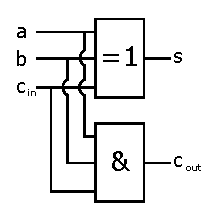
\includegraphics[height=.3\textheight]{Figurer/fa}
		\caption{A full adder.}
		\label{fig:fa} 
	\end{subfigure}%
	\begin{subfigure}{.5\textwidth}
		\centering
		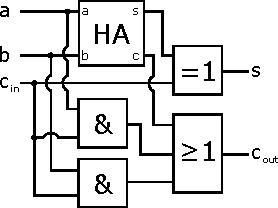
\includegraphics[height=.3\textheight]{Figurer/fa2}
		\caption{A full adder using a half adder.}
		\label{fig:fa2} 
  	\end{subfigure}
	\caption{Figure~\ref{fig:fa} shows the data flow implementation of a full adder,
		and Figure~\ref{fig:fa2} shows the alternative structural design using a half adder.}
\end{figure}

\newpage

\subsection{Top-level Design}

The top-level design consists of a number of components, such as registers, memory units, ALU's
and multiplexers. What we did was to design these components and then in the end, we connected
them with each other in the data path.

The register is implemented using a D-flip-flop and a 2-to-1 multiplexer. The {\it WE} is the select
signal for the multiplexer and it chooses what should be stored in the flip-flop, which is either
the already stored data or the input data ({\it DATA\_IN}). The register is implemented
generically so that words of any size can be stored. The memory unit consists of an arbitrary number
of registers, also using generic implementation. In the following picture, we can see what happens
when we read and write data to a memory unit:

\begin{figure}[h!]
	\centering
	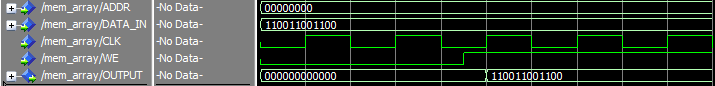
\includegraphics[width=1\textwidth]{Figurer/data_memory}
	\label{fig:sim}
\end{figure}

The memory is initially stored with the value `0' (or ``000000000000'' in binary) in address `0'.
{\it WE} is also low, which means writing is disabled. When {\it WE} becomes active, the word
``110011001100'' is stored at the next rising edge of the clock ({\it CLK}) signal.

The bus is implemented using a 4-to-1-multiplexer rather than using tri-state buffers. In this
way, no signals can overload, but there may be multiple select signals active. For this we have
the error signal ({\it ERR}), that activates when at least two select signals are active. The
select signal for the multiplexer and the {\it ERR}-signal are implemented using data flow, where
minimizations of the boolean expressions have been made (see Figure~\ref{fig:enc}).

\begin{figure}[h!]
	\centering
	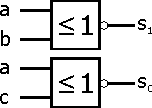
\includegraphics[width=.3\textwidth]{Figurer/enc4b}
	\caption{The minimized gate logic for the select signals of the bus multiplexer.}
	\label{fig:enc}
\end{figure}

\subsection{Controller}

\begin{figure}[h!]
	\centering
	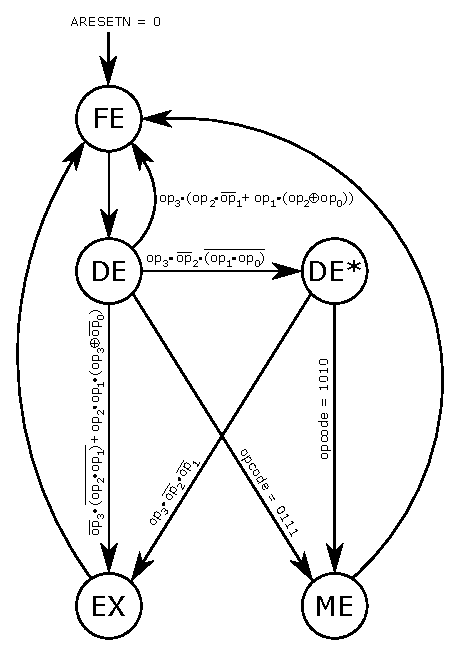
\includegraphics[width=0.5\textwidth]{Figurer/procController_FSM_Mealy}
	\caption{The {\it Final State Machine} of the processor's controller.}
	\label{fig:fsm}
\end{figure}


We divided the controller into three processes; the state combinatorial, state register and
the output combinatorial. In the state combinatorial we took the boolean expression for each 
state and minimized it through Karnaugh diagrams. The finite state machine is implemented in 
mealy state style so the states are dependent on both the current state and the opcode. 
State register has an asynchronous reset which restores the machine state to fetch ({\it FE}). 
The register is controlled by the \emph{master load enable} signal. The output combinatorial 
handles all the control signals. It is minimized in the same manner as the finite state machine.

\begin{figure}[h!]
	\centering
	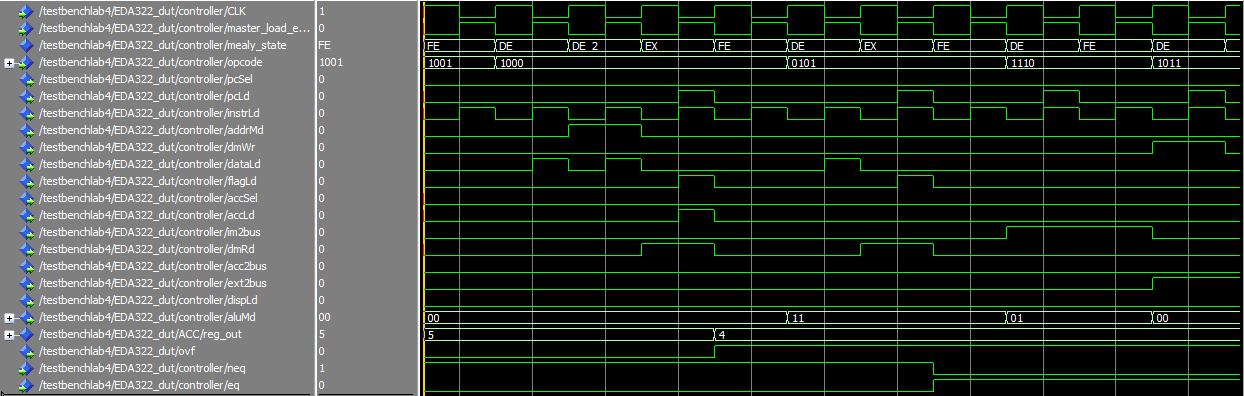
\includegraphics[width=1\textwidth]{Figurer/controller}
	\caption{Waveform of controller executing some instructions.}
	\label{fig:con}
\end{figure}
\newpage
In figure~\ref{fig:con} we have included a few waveforms showing the processor adding something 
from the memory to the accumulator and then comparing it to another memory cell. It then jumps 
depending on the result of the comparison. From the state we're in the accumulator holds the value 5. 
The instruction to be executed is ADX ACC, DM[DM[4]] which is an indirect addition. The data in the 
memory location is 255, so when the ALU performs the addition the accumulator stores the value 4 and 
we get an overflow. The next instruction, \emph{CMP ACC, DM[8]}, compares the value in the accumulator 
with the value in the memory location. In this case they are both 4 so the EQ signal is set to 1 and 
NEQ is set to 0. When we go to the next instruction, which is JNE 255, we will not jump because NEQ is 
set to 0.

\subsection{Processor's Testbench}

In the testbench we used behavioral VHDL to test our code. We used a reading function to read files which
contained expected outputs for each segmented display. In the architecture we divided all the testing 
of the displays into separate processes. In each process we assert that when a value changes in the display
it is equal to the expected output in the read file. If the assertion fails, the test exits immediately 
with an error message. Inputs were generated by initiating the memory units with the provided memory files.
Then in the test code we added a clock process so that the program could execute.

When we ran the testbench, we saw that we didn't get the expected output. We compared with the
{\it code\_to\_test.txt} file to see where it went wrong. We found out that in the data path,
there were some internal signals that weren't connected to the right modules, leading to unwanted
behaviour. This ultimately solved the problem and the testbench completed successfully.

\subsection{ChAcc on Nexys 3 board}

In this laboration, we programmed the Nexys 3 board with our code for the processor. The board
included switches and segmented displays that we used to test the correctness of our implementation.
The switches controlled what should be displayed on the two pairs of displays that were available.
We set it to show the data output, and the instruction operation code combined with the flags.
One switch was used for setting/resetting the clock signal, in order to step the program at an
appropriate speed. Table~\ref{tab:fib} shows the sequence of opcode values (we didn't care about
the flags) that were observed on the display while stepping through the program.
Table~\ref{tab:fib_data} shows the data that the program produces, which is indeed the beginning
of the fibonacci sequence. All the observed values matched with the simulation of the processor's
testbench in ModelSim (the same program was used for testing in the simulation).
   
\begin{table}   
	\centering
	\small
	\def\arraystretch{1.1}              
	\begin{tabular}{|l|l|l|}
		\hline
		PC & {\it Opcode}    & {\bf Assembly} \\ \hline
		0  & 0110 (6)        & LD ACC, DM[1]  \\
    1  & 0001 (1)        & AD ACC, DM[0]  \\
    2  & 1111 (F)        & DS             \\
    3  & 0111 (7)        & SB DM[1], Acc  \\
    4  & 0010 (2)        & SU Acc, DM[0]  \\
    5  & 0111 (7)        & SB DM[0], Acc  \\
    6  & 1100 (C)        & J 0            \\ \hline
	\end{tabular}
	\caption{The program is calculating the fibonacci sequence by continiously adding and storing
           two numbers in memory locations 0 and 1.}
	\label{tab:fib}
\end{table}

\begin{table}   
	\centering
	\small
	\def\arraystretch{1.1}              
	\begin{tabular}{|l|l|l|}
		\hline
		Display value & Decimal representation \\ \hline
		02  & 2                                \\
    03  & 3                                \\
    05  & 5                                \\
    08  & 8                                \\
    0D  & 13                               \\
    15  & 21                               \\
    22  & 34                               \\
    37  & 55                               \\
    59  & 89                               \\
    90  & 144                              \\    
    E9  & 233                              \\ \hline
	\end{tabular}
	\caption{The data produced by the program.}
	\label{tab:fib_data}
\end{table}

\subsection{Performance, Area and Power Analysis}
(max: 2 pages)
\\\\
For task 1 we tried to optimize our design for maximum performance with no regard to area usage or power consumption. We set the design goal to Balanced. In synthesis properties we set the optimization mode to Speed, optimization level to high and unchecked everything that tried to save power. We started with the timing constraint set at 7.000ns and lowered it further and further until the clock frequency was no longer improving. Then we lowered the time constraint a bit more, with no improvement. Our best clock frequency, 198.491 MHz, was achieved when meeting the timing constraint set at 5.100ns. The critical path is between fetch/decode and flag registers.

For task 2 we set the design goal to area reduction. In synthesis properties we set optimization mode to Area and optimization level to normal. We did not use any power saving options. We did manage to reduce the area used quite a bit compared to task 1. 

For task 3 we set the design goal to power optimization. In synthesis properties we set optimization mode to Area, optimization level to High, power to yes and global optimization to Maximum Delay. This configuration yielded less power consumption than task 1 and 2.
We found that the most power hungry module across all implementations is the ALU, followed by FE.

Task 1 was our most powerful design, but when we tried to maximize efficiency in task 4 we ended up with a result that was not only the most efficient yet but also had less area usage than task 2 and less power consumption than task 3. For this reason we ended up with only two different configurations. One optimized for performance and one for everything else. To achieve this result we used the design goal Minimum Runtime, the synthesis properties optimization mode Area, optimization level High, power to Yes and the map properties power Extra Effort and global optimization Power. The critical path with this configuration is from controller/mealy\_state\_FSM\_FFd1 to FReg/reg\_out\_2, which differs from the critical path in the other implementation.


\begin{table}   
	\centering
	\small
	\def\arraystretch{1.1}              
	\begin{tabular}{|l|l|l|}
		\hline
		{\bf Design Goals \& Strategies} & \bf Performance  & \bf Efficiency/Area/Power \\ \hline
		Design goal       & Balanced   & Minimum Runtime     \\ \hline
		{\bf Synthesis properties} & & \\ \hline
		-opt\_mode         & Speed & Area    \\
		-op\_level         & High & High   \\ 
		-power            & no   & yes  \\ 
		-glob\_opt         & AllClockNets & AllClockNets  \\ \hline
		{\bf Map properties} & &   \\ \hline
		-power            & off  & Extra Effort   \\ 
		-glob\_opt         & off  & off \\ \hline
	\end{tabular}
	\caption{Settings for the best implementations.}
	\label{tab:set}
\end{table}

\section{Analysis}
(max: 1 page)
\\\\
Summarize your results after performing all the labs (2, 3, 4 and 5).

Mention and discuss interesting findings and observations, as well as difficulties in completing some of the tasks of the four last labs.

After looking at your results, draw conclusions and describe briefly the learning outcome, that is what have you learnt by performing these labs?  

% Appendix
\newpage
\begin{appendix}

\section{Figures}
\label{app:fig}

\begin{figure}[h!]
 	\centering
	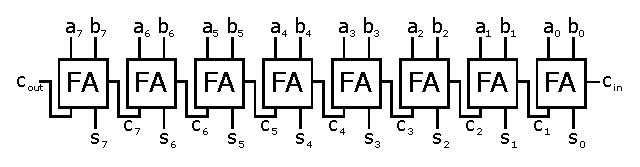
\includegraphics[width=1\columnwidth]{Figurer/rca}
  	\caption{A structural implementation of an 8-bit ripple carry adder using eight full adders.}
  	\label{fig:rca}
\end{figure}

\begin{figure}[h!]
 	\centering
	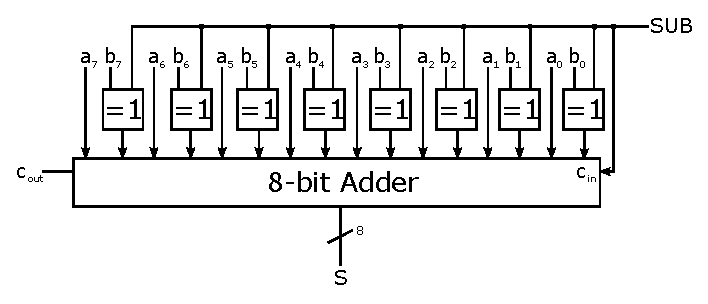
\includegraphics[width=1\columnwidth]{Figurer/sub}
  	\caption{Additional circuitry that is needed in order for the subtraction
		operation to work.}
  	\label{fig:sub}
\end{figure}

\end{appendix}

\end{document}
